\chapter{Linear Models: Regression}
\label{ch:regress}

Aims of this chapter\footnote{Here you work with the script file {\tt regress.R}}:

\begin{compactitem}
	\item More functions for plotting data and models.
	\item Calculating correlation coefficients.
	\item Fitting a regression model and significance testing.
	\item Using diagnostic plots to assess model suitability.
\end{compactitem}

As with the previous chapter, we'll start with creating a new blank 
script for you to fill in during the practical. We'll also be using the 
genome size data again, so:

\begin{compactitem}[$\quad\star$]
	\item Open R and change to the {\tt code} directory.
	\item Create a new blank script called `Regression.R' and add some 
	introductory comments.
	\item Add code to your script to load the genome size data into R and 
	check it.
\end{compactitem}

\section{Exploring the data}

In previous chapters we used {\tt plot} to create a scatterplot between 
two variables. If you have a set of variables to explore, writing code 
for each plot is tiresome, so R provides a the function {\tt pairs}, 
which creates a grid of scatterplots between each pair of variables. 
All it needs is a dataset.

\begin{compactitem}[$\quad\star$]
	\item Add {\tt pairs(genome, col=genome\$Suborder)} into your script 
	and run the code. 
\end{compactitem}

The result is messy! There are far too many variables in {\tt genome} 
for this to be useful. We need to cut down the data to fewer variables. 
In Chapter \ref{ch:ExpDesign}, we used indices to select colours; here, we can use 
indices to select columns from the data frame. This again uses square 
brackets ({\tt x[ ]}), but a data frame has two dimensions, rows and 
columns, so  you need to provide an index for each dimension, separated 
by commas. If an index is left blank, then all of that dimension (i.e. 
all rows or columns) are selected. Try the following to re-acquaint 
yourself to access data frame content using indices:  

\begin{lstlisting}
# create a small data frame:
> dat <- data.frame(A = c("a", "b", "c", "d", "e"), B = c(1, 2, 3, 4, 5))
> dat[1, ] # select row 1 (all columns selected)
	A B
1 a 1

> dat[, 2] # select column 2 (all rows selected)
[1] 1 2 3 4 5
> dat[2, 1] # select row 2, column 1
[1] "b"

\end{lstlisting}

Now let's get started with the actual analysis. We will look at five 
key variables: genome size, body weight, total length, forewing length 
and forewing area. If you look at the output of {\tt str(genome)}, 
you'll see that these are in columns 4, 7, 8, 12 and 14. We can record 
the indices of these columns and use this to select the data in the 
pairs plot.

\begin{lstlisting}
morpho <- c(4, 7, 8, 12, 14)
pairs(genome[, morpho], col = genome$Suborder)	
\end{lstlisting}

\begin{compactitem}[$\quad\star$]
	\item Add the code above to your script and run it
\end{compactitem}

The {\tt pairs} plot should give you something like the plot below:

\begin{center}
	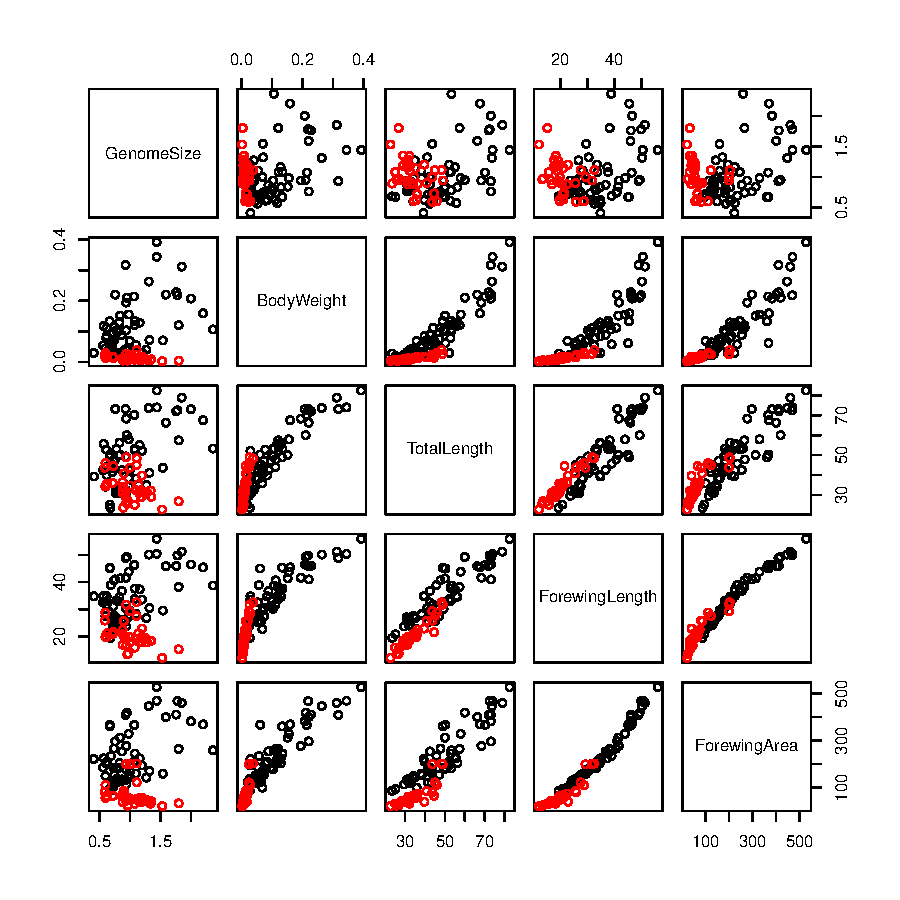
\includegraphics[width=\textwidth]{pairs.pdf} 
\end{center}

Each scatterplot is shown twice, with the variables swapping between 
the $x$ and $y$ axes. You can see immediately that the relationships 
between the four morphological measurements and genome size are fairly 
scattered but that the plots comparing morphology show much clearer 
relationships.

\section{Correlations}

One way of summarising how close strong the relationship between these 
variables are is to calculate a correlation coefficient. Pearson 
correlations look at the difference of each point from the mean of each 
variable (and since it uses means, it is a parametric statistic). 

It is calculated using of the differences from the mean on each axis. 
The key calculation is --- for each point -- to get the product of the 
differences on each axis and add them up. If the points are mostly top 
left ($-x$, $y$) or bottom right ($x$, $-y$) then these products are 
mostly negative ($-xy$); if the points are mostly top right ($x$, $y$) 
or bottom left ($-x$, $-y$) then the products are mostly positive 
($xy$).  

\begin{center}
	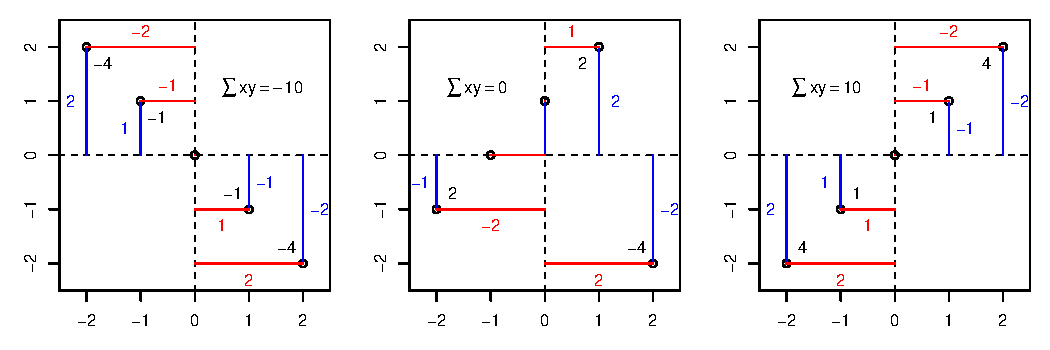
\includegraphics[width=\textwidth]{corr.pdf} 
\end{center}

The plots above show three clear cases where all the values of $xy$ are 
negative or positive or where both are present and sum to zero. The 
Pearson correlation coefficient simply scales these sums of $xy$ to be 
between -1 (perfectly negatively correlated) and 1 (perfectly 
positively  correlated) via zero (no correlation).

We will use two functions to look at correlations. The first is {\tt 
cor}, which can calculate correlations between pairs of variables, so 
is a good partner for {\tt pairs} plots. The second is {\tt cor.test}, 
which can only compare a single pair of variables, but uses a $t$ test 
to assess whether the correlation is significant. 

\begin{compactitem}[$\quad\star$]
	\item Try the following (and include it in your R script file)
\end{compactitem}


\begin{lstlisting}
> cor(genome[, morpho], use = "pairwise")
\end{lstlisting}

You should see a correlation matrix. Then,

\begin{lstlisting}
> cor.test(genome$GenomeSize, genome$TotalLength, use = "pairwise")	

Pearson's product-moment correlation

data: genome$GenomeSize and genome$TotalLength
t = 3.551, df = 96, p-value = 0.0005972

alternative hypothesis: true correlation is not equal to 0 
95 percent confidence interval:
  0.1526 0.5050 
sample estimates:
    cor 
 0.3407   
\end{lstlisting}

The {\tt use='pairwise'} in the above tells R to omit observations with 
missing data and use complete pairs of observations. The first function 
confirms our impressions from the graphs: the correlations between 
genome size and morphology are positive but comparatively weak and the 
correlations between morphological measurements are positive and very 
strong (i.e. close to 1). The correlation test tells us that genome 
size and body length are positively correlated (r=0.34, $t$ = 3.5507, 
df = 96, $p$ = 0.0006).

\begin{compactitem}[$\quad\star$]
	\item Again, remember this example when reporting correlations!
\end{compactitem}

\section{Transformations and allometric scaling}

There is one problem with the correlations above: {\it correlations 
assume a straight line relationship}. Some of the scatterplots above 
are fairly straight but there are some strongly curved relationships. 
This is due to the allometric scaling mentioned in Chapter \ref{ch:ExpDesign}: two of 
the variables are in linear units (total and forewing length), one is 
in squared units (forewing area) and one in cubic units (body weight, 
which is approximately volume).

The relationships between these variables can be described using a 
power law: $y = ax^b$. Fortunately, if we log transform this equation, 
we get $\log(y) = \log(a) + b \log(x)$. This is the equation of a 
straight line ($y=a+bx$), so we should be able to make these plots 
straighter by logging both axes. We saw in Chapter \ref{ch:ExpDesign} that we can 
create a new logged variable in the data frame like this:

\begin{lstlisting}
> genome$logGS <- log(genome$GenomeSize)
\end{lstlisting}

\begin{compactitem}[$\quad\star$]
	\item Using this line as a template, create a new logged version of 
	the five variables listed above.
	\item Using {\tt str}, work out which column numbers the logged 
	variables are and create a new variable called {\tt logmorpho} 
	containing these numbers.
	\item Copy the {\tt pairs} and {\tt cor} test from earlier in your 
	script and modify them to run these functions for the columns given 
	in {\tt logmorpho}.
\end{compactitem}

The correlations should give the following output:
\begin{lstlisting}
> cor(genome[, logmorpho], use = "pairwise")

         logGS   logBW  logTL  logFL   logFA
 logGS 1.00000 0.08406 0.2224 0.1150 0.06808
 logBW 0.08406 1.00000 0.8892 0.9456 0.94996
 logTL 0.22244 0.88919 1.0000 0.9158 0.86207
 logFL 0.11500 0.94565 0.9158 1.0000 0.97916
 logFA 0.06808 0.94996 0.8621 0.9792 1.00000
\end{lstlisting}

The scatterplots should look like this and show that logging the data 
has very successfully removed allometric scaling effects in the data:
\begin{center}
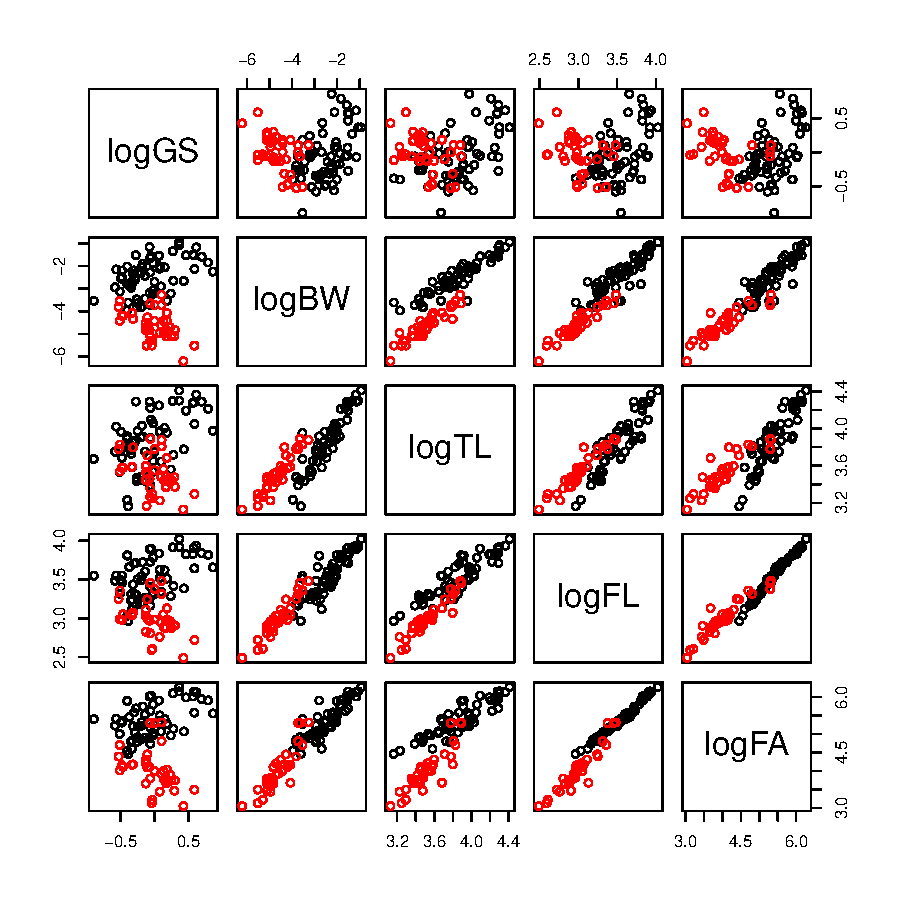
\includegraphics[width=\textwidth]{pairsLog.pdf} 
\end{center}

\section{Regression}

We'll now look at fitting the first linear model of this course, to 
explore whether log genome size explain log body weight. The first 
thing to do is to plot the data:

\begin{center}
	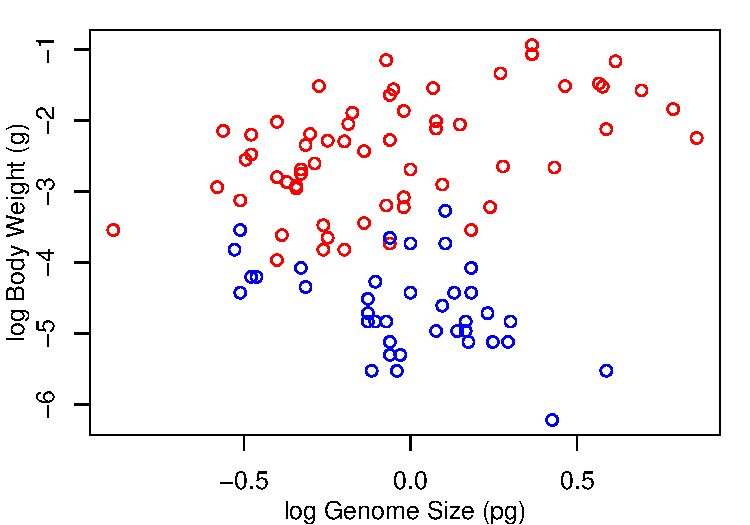
\includegraphics[width=0.5\textwidth]{gsVbw.pdf} 
\end{center}

It is clear that the two suborders have very different relationships: 
to begin with we will look at dragonflies (Anisoptera). We will 
calculate two linear models:

\begin{compactdesc}
	\item [The null model] This is the simplest linear model: nothing is 
	going on and the response variable just has variation around the 
	mean: $y = \beta_1$. This is written as an R formula as {\tt y 
	\textasciitilde{} 1}.
	\item [Linear regression] This models a straight line relationship 
	between the response variable and a continuous explanatory variable: 
	$y= \beta_1 + \beta_{2}x$.
\end{compactdesc}

The code below fits these two models.

\begin{lstlisting}
> nullModelDragon <- lm(logBW ~ 1, data = genome, subset = Suborder == 
"Anisoptera")
> genomeSizeModelDragon <- lm(logBW ~ logGS, data = genome, subset = 
Suborder == "Anisoptera")
\end{lstlisting}

\begin{compactitem}[$\quad\star$]
	\item Note the long names for the models. Short names are easier to 
	type but calling R objects names like {\tt mod1},  {\tt mod2},  {\tt 
	xxx} swiftly get confusing!   
	\item Enter these models into your script and run them.
\end{compactitem}

Now we want to look at the output of the model. Remember from the 
lecture that a model has {\it coefficients} (the $\beta$ values in the 
equation of the model) and {\it terms} which are the explanatory 
variables in the model. We'll look at the {\it coefficients} first:

\begin{lstlisting}
> summary(genomeSizeModelDragon) 
 Call:
 lm(formula = logBW ~ logGS, data = genome, subset = Suborder == 
     "Anisoptera")
 
 Residuals:
    Min     1Q Median     3Q    Max 
 -1.324 -0.612  0.097  0.519  1.324 
 
 Coefficients:
             Estimate Std. Error t value Pr(>|t|)    
 (Intercept)  -2.3995     0.0908  -26.41  < 2e-16 ***
 logGS         1.0052     0.2398    4.19  9.5e-05 ***
 ---
 Signif. codes:  0 '***' 0.001 '**' 0.01 '*' 0.05 '.' 0.1 ' ' 1 
 
 Residual standard error: 0.697 on 58 degrees of freedom
   (2 observations deleted due to missingness)
 Multiple R-squared: 0.233,	Adjusted R-squared: 0.219 
 F-statistic: 17.6 on 1 and 58 DF,  p-value: 9.54e-05  
\end{lstlisting}

There is a lot of information there: the model description (`{\tt 
Call}'), a summary of the residuals, a table of coefficients and then 
information on residual standard error, r squared and an $F$ test. All 
of these will become clearer during this course --- for the moment, 
concentrate on the coefficients table.

There are two rows in the coefficient table, one for each coefficient 
in $y=\beta_1 + \beta_2x$ --- these are the intercept and the slope of 
the line. The rest the details on each row are a $t$ test  of whether 
the slope and intercept are significantly different from zero. 

Now we will look at the {\it terms} of the model using the {\tt anova} 
function. We will have a proper look at ANOVA (Analysis of Variance) in 
chapter \ref{ch:ANOVA}. Meanwhile, for our current purposes, all you need to 
know is that ANOVA tests how much variation in the response variable is 
explained by each explanatory variable. We only have one variable and 
so there is only one row in the output:

\begin{lstlisting}
> anova(genomeSizeModelDragon)

 Analysis of Variance Table
 
 Response: logBW
           Df Sum Sq Mean Sq F value  Pr(>F)    
 logGS      1   8.53    8.53    17.6 9.5e-05 ***
 Residuals 58  28.14    0.49                    
 ---
 Signif. codes:  0 '***' 0.001 '**' 0.01 '*' 0.05 '.' 0.1 ' ' 1 
\end{lstlisting}

This table is comparing the variation in log body weight explained by 
log genome size to the total variation in log body weight. We are 
interested in how much smaller the residuals are for the genome size 
model than the null model. Graphically, how much shorter are the red 
residuals than the blue residuals:

\begin{center}
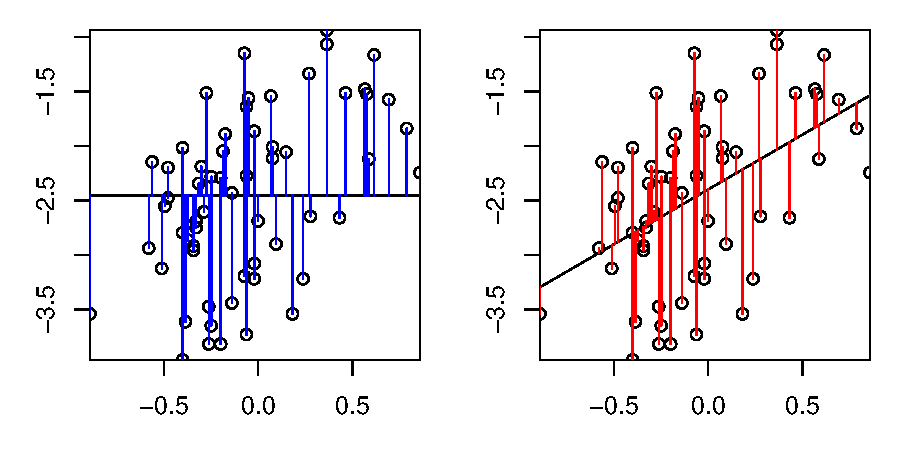
\includegraphics[width=0.8\textwidth]{regResid.pdf} 
\end{center}

We can get the sums of the squares of these residuals from the two 
models using the function {\tt resid}, and then square them and add 
them up:

\begin{lstlisting}
> sum(resid(nullModelDragon) ^ 2)
 [1] 36.67
 
> sum(resid(genomeSizeModelDragon) ^ 2)
 [1] 28.14
\end{lstlisting}

So we have five columns in the table:
\begin{compactdesc}
	\item[Df] This shows the degrees of freedom. Each fitted parameter/coefficient takes up 
	a degree of freedom from the total sample size, and the left over are the residuals degree of freedom. In this 
	case, genome size adds a slope (compare the null model $y=\beta_1$ 
	and this model $y=\beta_1 + \beta_2x$ --- there is one more $\beta$). 
	\item[Sum Sq] This shows sums of squares. The bottom line is the 
	residual sum of squares for the model and the one above is the 
	variation explained by genome size. Using the two values from above, 
	the sums of square residuals for the null model are 36.67. In the 
	genome size model, the sum of square residuals are 28.14 and so 
	$36.67-28.14=8.53$ units of variance have been explained by this 
	model.
	\item[Mean Sq] These are just the Sum Sq (Sum of Squares) values divided by the 
	degrees of freedom. The idea behind this is simple: if we explain 
	lots of variation with one coefficient, that is good (the null model), and if we explain a 
	small amount of variation with a loss of degree of freedom (by adding and then estimating more parameters), then that is bad.
	\item[F value] This is the ratio of the Mean Sq for the variable and 
	the residual Mean Sq. This is used to test whether the explained 
	variation is large or small.
	\item[Pr(>F)] This is a $p$ value --- the probability of the variable 
	explaining this much variance by chance. 
\end{compactdesc}

In this case, it is clear that genome size explains a significant 
variation in body weight. 

\begin{compactitem}[$\quad\star$]
	\item Include the {\tt summary} and {\tt anova} commands for {\tt 
	genomeSizeModelDragon} in your script, run them and check you are 
	happy with the output.
	\item Using this code as a template, create a new model called {\tt 
	genomeSizeModelDamsel} that fits log body weight as a function of log 
	genome size for damselflies.
	\item Write and run code to get the  {\tt summary} and {\tt anova} 
	tables for this new model.
\end{compactitem}

\section{Plotting the model}

Now we can plot the data and add lines to show the models. For simple 
regression models, we can use the function {\tt abline(modelName)} to 
add a line based on the model.
\begin{compactitem}[$\quad\star$]
 \item You already know how to create and customise scatterplots from 
 previous chapters. Create a plot of log body weight as a function of 
 log genome size, picking your favourite colours for the points.
 \item Use {\tt abline} to add a line for each model and use the {\tt 
 col} option in the function to colour each line to match the points. 
 For example: {\tt abline(genomeSizeModelDragon, col='red')}.
\end{compactitem}

You should get something like Figure \ref{fig:GenoRegModels}.

\begin{figure} \centering
	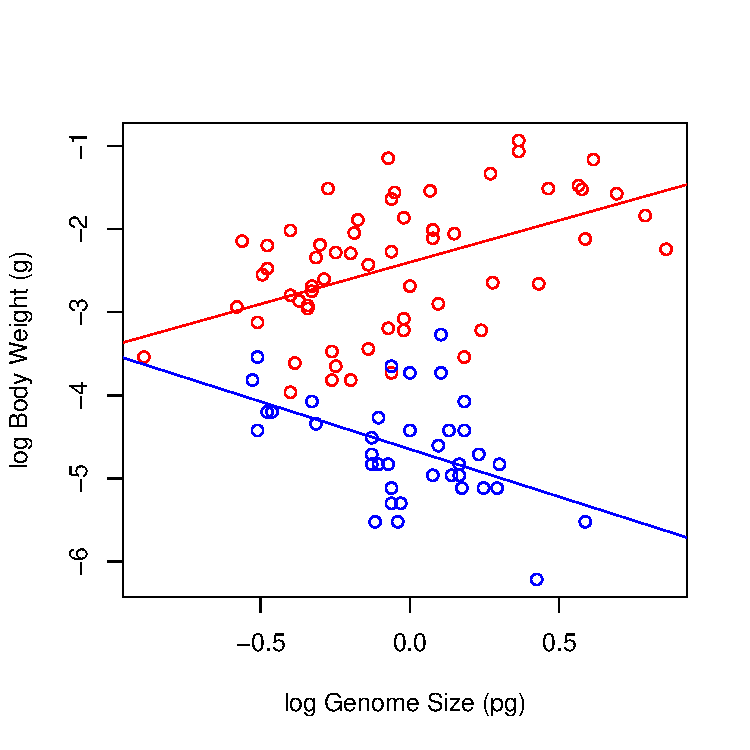
\includegraphics[width=0.5\textwidth]{GenoRegModels.pdf}
	\caption{Linear regression models fitted to the body weight vs. 
	genome size to the Dragonfly (red) and Damselfly (blue) subsets of 
	the data.}
	\label{fig:GenoRegModels}
\end{figure}

\section{Model diagnostics}

Now that we have our models, we need to check that they are appropriate 
for the data. For this, we will inspect ``diagnostic plots''. Producing 
diagnostic plots is easy in R --- if you {\tt plot} a model, then R 
produces a set of diagnostic plots! 

\begin{compactitem}[$\quad\star$]
	\item Try the following code (and include in the R script file):
\end{compactitem}
\begin{lstlisting}
> par(mfrow = c(2, 2), mar = c(5, 5, 1.5, 1.5))
> plot(genomeSizeModelDragon)
\end{lstlisting}
This should give the plots shown in figure \ref{fig:DiagModDragon}.
\begin{figure} \centering
	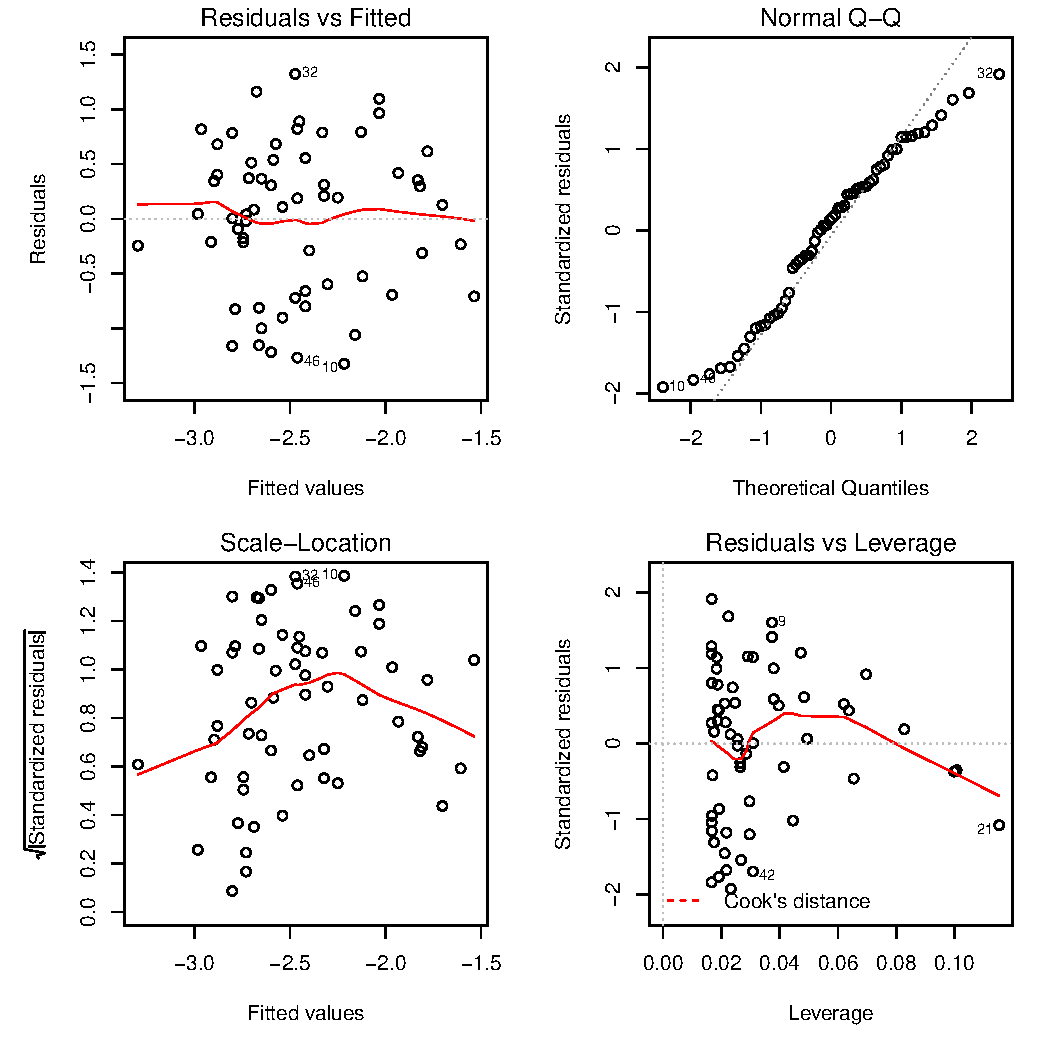
\includegraphics[width=0.7\textwidth]{DiagModDragon.pdf}
	\caption{Diagnostics for the {\tt lm} fit to the Dragonfly data 
	subset.}
	\label{fig:DiagModDragon} 
\end{figure}
And,
\begin{lstlisting}
> par(mfrow = c(2, 2), mar = c(5, 5, 1.5, 1.5))
> plot(genomeSizeModelDamsel)
\end{lstlisting}
This should give the plots shown in figure \ref{fig:DiagModDamsel}.

\begin{figure}\centering
	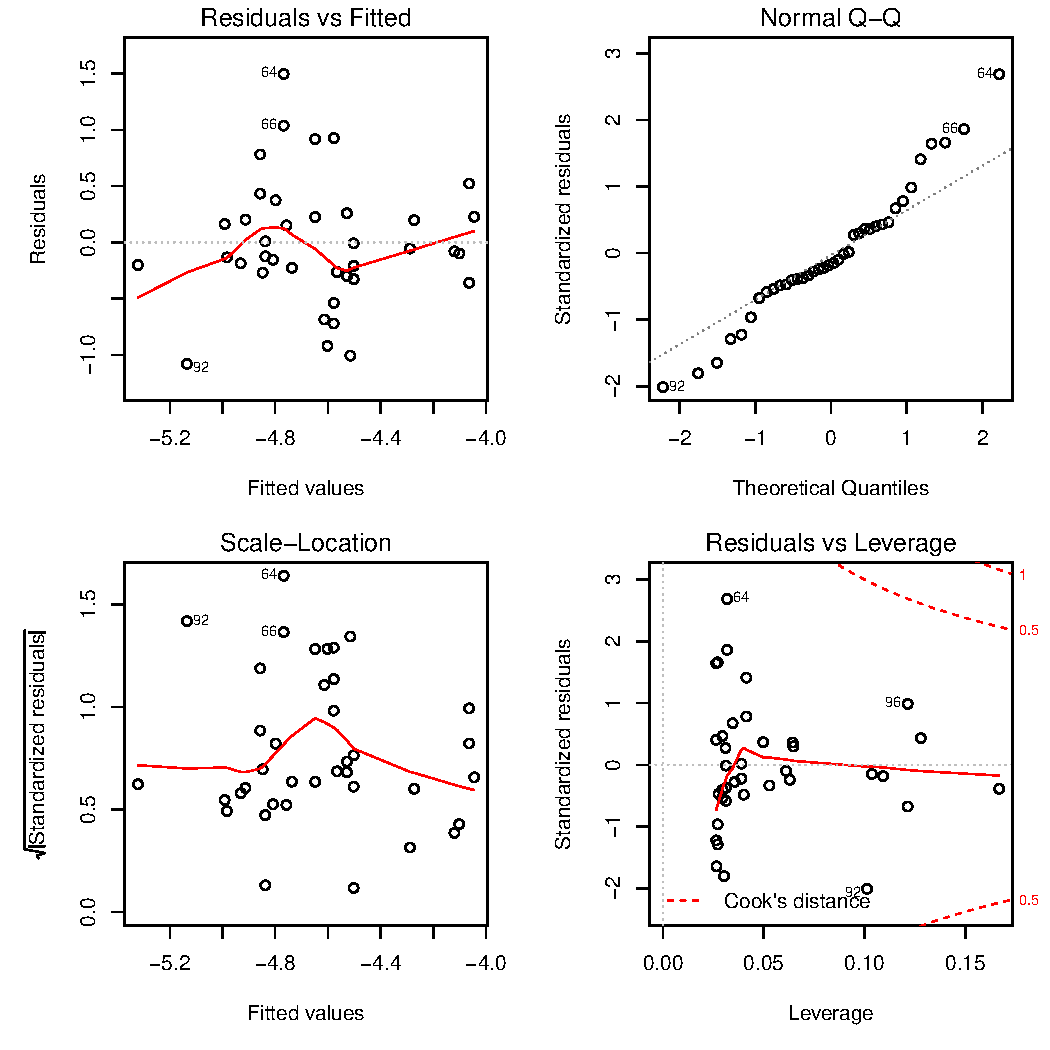
\includegraphics[width=0.7\textwidth]{DiagModDamsel.pdf}
	\caption{Diagnostics for the {\tt lm} fit to the Damselfly data 
	subset.}
	\label{fig:DiagModDamsel} 
\end{figure}

The diagnostic plots are:
\begin{compactdesc}
		
		\item[Residuals vs Fitted] This plot is used to spot if the 
		distribution of the residuals (the vertical distance from a point 
		to the regression line) has {\it similar variance} for different 
		predicted values (the y-value on the line corresponding to each 
		x-value). There should be no obvious patterns (such as curves) or 
		big gaps. If there was no scatter, if all the points fell exactly 
		on the line, then all of the dots on this plot would lie on the 
		gray horizontal dashed line. The red line is a smoothed curve to 
		make it easier to see trends in the residuals. It is flat in the 
		Dragonfly model fit (Figure \ref{fig:DiagModDragon}), and a bit 
		more wavy than we would like in the in the Damselfly model fit 
		(Figure \ref{fig:DiagModDamsel}), but there are no clear trends in 
		either, which is what you hope to see. 
		
		\item[Normal Q--Q] This plot is to check whether the residuals are 
		{\it normally distributed } --- are the values of the observed 
		residuals similar to those expected under a normal distribution? 
		Ideally, the points should form a perfectly straight line, 
		indicating that the observed residuals exactly match the expected. 
		Here, note that the points lie pretty close to the dashed line in 
		both Figures \ref{fig:DiagModDragon} \& \ref{fig:DiagModDamsel}, 
		but deviate at the ends, especially for Damselflies. However, some 
		deviation is to be expected near the ends --- here these deviations 
		are just about acceptable.

		\item[Scale--Location] The x-axis on this plot is identical to the 
		Residuals vs Fitted plot -- these are the fitted values. The y-axis 
		is the square root of the {\it standardized residuals}, which are 
		residuals rescaled so that they have a mean of zero and a variance 
		of one. As a result, all y-axis values are positive. Thus large 
		residuals (both positive and negative) plot at the top, and small 
		residuals plot at the bottom (so only their {\it scale} is 
		retained). Thus, all of the numbered points (which will be the same 
		in all plots) plot at the top here. The red line here shows the 
		trend, just like the Residuals vs Fitted plot. The regression 
		analysis has assumed homoscedasticity, that the variance in the 
		residuals doesn't change as a function of the predictor. If that 
		assumption is correct, the red line should be relatively flat. It 
		is not quite as flat as we would like, especially for the Dragonfly 
		analysis (Figure \ref{fig:DiagModDragon}).
		
		\item[Residuals vs Leverage] This plot shows the standardized 
		residuals against leverage. ``Leverage'' is a measure of how much 
		each data point influences the linear model's coefficient 
		estimates. Because the regression line must pass through the 
		centroid (``pivot point'') of the data (Figure \ref{fig:Leverage}), 
		points that lie far from the centroid have greater leverage, and 
		their leverage increases if there are fewer points nearby. There 
		are two key things to note about this plot:
		\begin{figure} \centering
			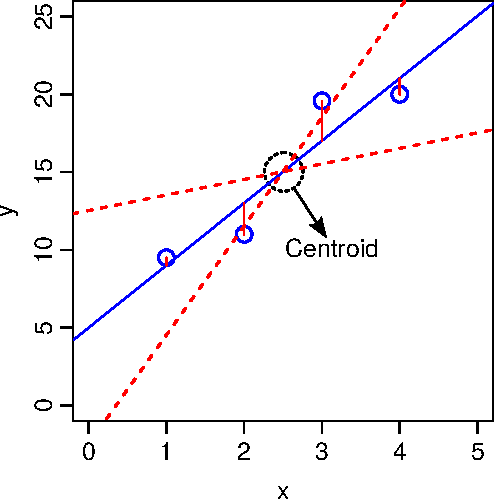
\includegraphics[width=0.4\textwidth]{Leverage.pdf}
			\caption{Leverage of data points on slope of a regression. The 
			points further away from the centroid in the x-axis direction 
			have more leverage, and can therefore move the regression line up 
			or down (dashed red lines).}
			\label{fig:Leverage} 
		\end{figure}

		\begin{enumerate}
			\item The standardized residuals (y-axis) are centered around 
			zero and reach 2-3 standard deviations away from zero. They 
			should also lie symmetrically about zero, as would be expected 
			for a normal distribution. This is the case for the Damselfly 
			plot (Figure \ref{fig:DiagModDamsel}) , but not so much for the 
			Dragonfly plot Figure \ref{fig:DiagModDragon}. 
			\item The contours values show {\it Cook's distance} (only 
			visible in the Damsefly plot), which measures how much the 
			regression would change if a point was deleted. Cook's distance 
			is increased by leverage and by large residuals: a point far from 
			the centroid with a large residual can severely distort the 
			coefficient estimates from the regression. On this plot, you want to see that the red smoothed 
			line stays close to the horizontal gray dashed line and that no 
			points have a large Cook's distance (i.e, >0.5). Both are true 
			here.
		\end{enumerate}
		This is an important diagnostic plot in regression analyses in 
		particular because it tells you whether your estimate of the slope 
		coefficient in particular is strongly affected by certain data 
		points.  

\end{compactdesc}
Note that certain points are numbered in all the plots --- these are 
points to pay special attention to because they are {\it potential} 
outliers. The numbers correspnd to the row number for that dataset in 
your data frame. You can easily identify these points in your data plot 
(Figure \ref{fig:GenoRegModels}) because the order of the points along 
the fitted values axis (y-axis) in the diagnostic plot matches the 
order along the x-axis in the data plot. So, fo example here, in Figure 
\ref{fig:DiagModDragon}, the two numbered points (46, 10) near the 
bottom correspond in the data plot (Figure \ref{fig:GenoRegModels}) to 
the two red points near the center-left that lie farthest below the red 
line.

Thus, neither the Drangonfly nor the Damselfly diagnostic plots look 
perfect, but this level of deviation from assumptions of linear models 
is acceptable. The main worrying factors are that the QQ plot for 
Damselflies indicates the observed residuals are a bit more extreme 
than expected, and the Scale--Location plot for Dragonflies suggests 
some pattern in the standardized residuals wrt location of the fitted 
values.

\begin{compactitem}[$\quad\star$]
 \item Copy the code to create the diagnostic plots into your script to 
 keep a record of the code and run it.
\end{compactitem}

\section{Reporting the model}

Now we know that the models are appropriate and we have a plot, the 
last thing is to report the statistics. For the damselfly model, here 
is one summary that would do: log genome size explains significant 
variation in log body weight in dameselflies (F=10.5, df=1,36, p=0.0025) 
and shows that body weight decreases with genome size (intercept: 
-4.65,  se=0.09; slope: -1.14, se=0.35).
